\documentclass[10pt,a4paper]{article}

% package for making the margins thinner
\usepackage[left=2cm, right=2cm, top=2cm, bottom=2cm]{geometry}

% I don't recall what this package was for
\usepackage[toc,page]{appendix}

\renewcommand{\baselinestretch}{1.15}
\usepackage{graphicx}
\graphicspath{{./images/}}


%\newcommand{\bigsize}{\fontsize{35pt}{20pt}\selectfont}
\begin{document}
\begin{titlepage}
    \title{INFO3406 Project Stage 1}
    \author{Linzi Zhu(460381996)\\
            \and
            Nick Zhou(460363707)
    }
    \date{September 2018}
    \maketitle
\end{titlepage}
    \begin{tableofcontents}
        \centering
        \tableofcontents
    \end{tableofcontents}
    \pagebreak

    \section{Section 1: Problem}
    Deciding on a name is often one of the difficult parts of any project, and for good reason. \
    The title is often the first thing any prospective member of your audience will interact \
    with before engagement, and as such everyone wants to pick the best one. Many names, particularly \
    in media, aren't constructed of whole cloth, but are formed from existing English words. And \
    these words have power, conveying emotions, feelings and attitudes - to varying degrees. Using \
    the PAD Emotional framework, it's possible to quantify exactly how much power each of the \
    constituent words in a title have. Combining this with existing movie data, it's possible \
    to classify the predicted emotional response to any given movie's title. Thus this project \
    aims to explore the extent to which a good name affects a movies box office ratings, specifically -

    \begin{enumerate}
        \item Is there a link between the emotional response a movie's title evokes (sight unseen) and the movies eventual gross revenue?
        \item Using these models, can we train a predictor to assess the value of a title for any given movie?

    \end{enumerate}

    \section{Section 2: Approach}
    The approach we are going to be taking in Stage 2 is performing statistical analysis on our dataset. We will attempt to \
    answer the questions we set out by doing explaratory factor analysis and t-tests.

    \section{Section 3: Data}

    For this dataset we combined 2 larger datasets, while trimming some extraneous information not relevant to this report. A 2011 report from the National Research Council Canada on Word-Emotion Association Lexicon - acquired from https://saifmohammad.com/WebPages/NRC-Emotion-Lexicon.htm, and the IMDB5000 movie dataset, listing a huge amount of metadata related to 5000 select movies - acquired from https://github.com/Godoy/imdb-5000-movie-dataset
    \newline \newline
    The Word-Emotion Association Lexicon was originally compiled by asking volunteers on Amazon's Mechanical Turk to rate a series of words, the total of which were analysed and compiled into the report by the NRC. In particular, we used the word to Valence, Arousal and Dominance report, which takes a large number of English unigrams and assigns to each a value from 0 to 1 for valence, arousal and dominance. In order -

    \begin{itemize}
        \item Valence (sometimes known as pleasure) measures how pleasant or unpleasant one feels about something. For instance both anger and fear are unpleasant emotions, and both score on the displeasure side. However joy is a pleasant emotion.
        \item Arousal measures how energized or soporific one feels. It is not the intensity of the emotion -- for grief and depression can be low arousal intense feelings. While both anger and rage are unpleasant emotions, rage has a higher intensity or a higher arousal state. However boredom, which is also an unpleasant state, has a low arousal value.
        \item Dominance represents the controlling and dominant versus controlled or submissive one feels. For instance while both fear and anger are unpleasant emotions, anger is a dominant emotion, while fear is a submissive emotion
    \end{itemize}

    The IMDB5000 is essentially a scrape of the IMDB database, the stats for which are all user compiled, like Wikipedia.
    \newline \newline
    In our report, we take a combination of these statistics. Firstly, the titles of the films in question, stored as strings. Then the gross revenue of the film as described my IMDB, stored as an integer. Finally, we took an average of each of the valence, arousal and dominance values of each word in the corresponding titles, represented as a real number from 0-1.
    \newline \newline
    We believe that using the VAD model we can analyse the effect that the emotional response the average person has to the title of a movie has on the film's final gross revenue.
    \newline \newline
    %\heading{tools}
    The tools we used were:

    \begin{itemize}
        \item python
        \item pgAdmin4
        \item SPSS
        \item Microsoft Excel
    \end{itemize}
    %\heading{cleaning}

    We began by cleaning to data for our purposes. The Lexicon data was divided into several different breakdowns, of which the Word by VAD report was of most interest to us, using real numbers (the other interesting report used Word by Affectation and Emotion, but used a boolean measure which proved non-useful for our purposes). This was formatted as a tab separated .txt file, so by porting it into Microsoft Excel, we exported the file as a CSV, ready to load into pgAdmin4.
    \newline \newline
    On the other hand, the IMDB5000 data had many, many more fields than necessary, including such information as 'Whether the movie was in colour or black and white' and 'How many faces were on the movie poster'. Already in .csv format, we loaded the data in Excel and manually removed all fields except title, language and gross. Then we removed all non-english films, so as not to throw off the lexical analysis by including films with english homographs (for instance, "Shin seiki Evangerion" includes the english word 'shin', but means 'new' in Japanese, which would affect our lexical analysis). Finally, I removed all films with an unrecorded gross revenue, so as not to have any blank fields. This produced the clean version of our movie metadata, which we also loaded into pgAdmin4.
    \newline \newline
    Then, using a specific SQL query (provided in the code report) we muxed the data, producing a list of ~4000 movie titles, along with their gross revenue and an average of the valence, arousal and dominance of every non-particle english word in their titles. This was the final CSV file for use in this analysis.
    \newline \newline

    Appendix A shows a series of histograms that count each average valance, arousal and \
    dominance scores of each title in our dataset. On average, the titles are left tailed,\
    indicating preference for pleasant over unpleasant. Conversely, the arousal graph is slightly\
    left tailed, indicating less arousing than not. The dominance graph follows a roughly\
    normal distribution, which affirms the min/max and sd tables that have been produced.
    \newline \newline
    Appendix B shows a series of scatter plots. The scatter plots were difficult to analyse \
    due to the difference between the majority of the body and how extreme the outliers are. \
    We will very likely have to produce a second series of grahs that disregard the outliers in \
    order to get a better sense of scale. The outliers don't seem to follow the same distribution \
    as the histograms would imply meaning there may be some interesting analysis in the future.

    \begin{appendices}
        \section{Graph 1}
        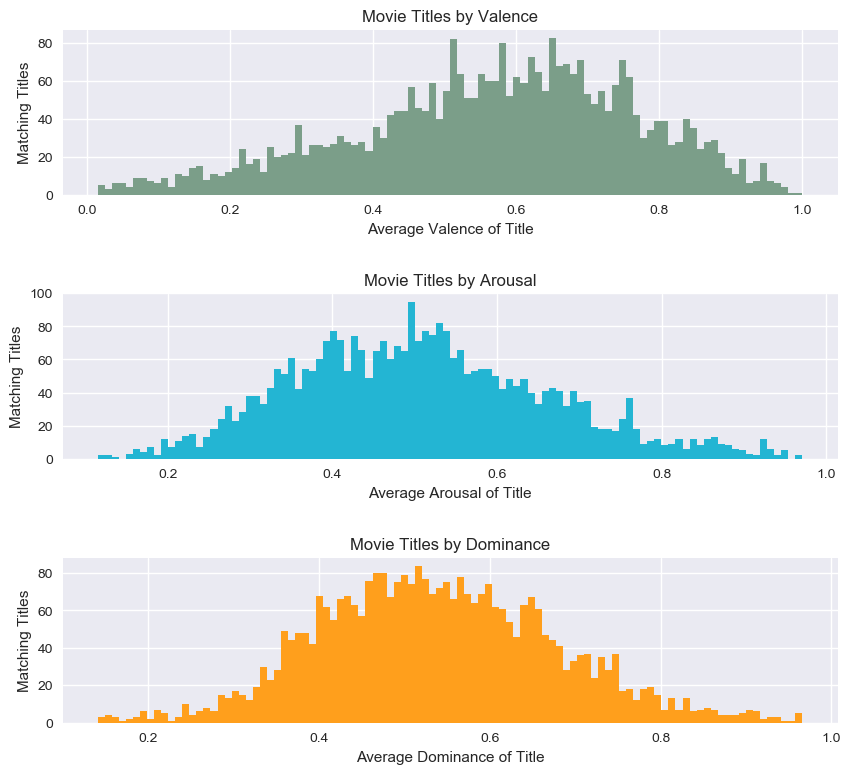
\includegraphics[scale=0.8]{Movie_titles_by_vad}
        \section{Graph 2}
        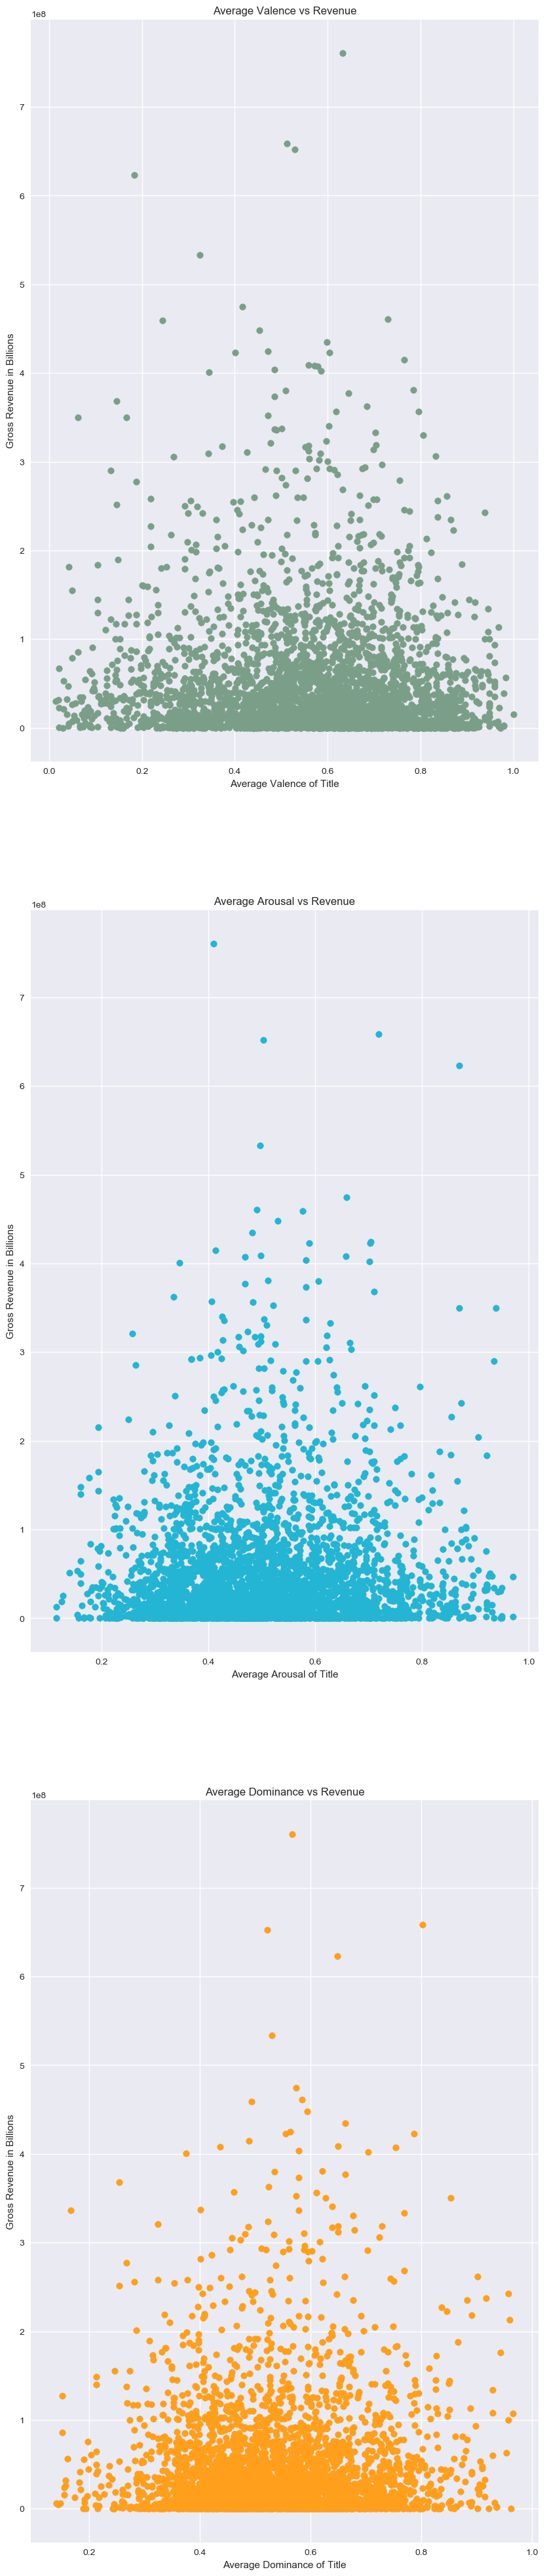
\includegraphics[scale=0.25]{vad_by_gross}
        %
        %\section{Something else}
        %Things that are not graphs will go here.
    \end{appendices}
\end{document}
